
\documentclass[conference]{IEEEtran}
\usepackage[T1]{fontenc}
\usepackage{amsmath,amssymb}
\usepackage{booktabs,tabularx,array}
\usepackage{graphicx}
\usepackage{tikz}
\usetikzlibrary{positioning,arrows.meta}
\usepackage{xurl}
\usepackage[hidelinks]{hyperref}
\usepackage{balance}
\title{API-Range-Aware Documentation Retrieval for Evolving npm Libraries: An Extended Implementation and Pilot Evaluation}
\author{\IEEEauthorblockN{Azmat Ullah}
\IEEEauthorblockA{Department of Computer Science, FAST-NUCES, Islamabad, Pakistan\\
Registration No.: 26i-7841\\
\texttt{\detokenize{i267841@isb.nu.edu.pk}}}}
\begin{document}
\maketitle
\begin{abstract}
Documentation-augmented code generation can fail when a retrieved example is relevant to a request but incompatible with an installed package version. This work extends a preliminary npm retrieval prototype with explicit API-validity intervals, controlled stable-API cases, paired statistical analysis, and an execution-ready generation workflow. We assemble a hand-curated test corpus of 39 documentation paraphrases and 42 version-conditioned tasks from Express, Mongoose, and React Router. Six retrieval conditions compare sparse BM25 and latent semantic analysis (LSA), each with no compatibility check, exact document-version matching, or manually annotated API-validity ranges. On the controlled corpus, BM25 correct-document Top-1 accuracy increases from 42.9\% without filtering to 66.7\% with either compatibility constraint. For LSA, the corresponding values are 35.7\% and 57.1\%. The range-aware method recovers more designated stable-API documents than exact matching but provides no overall Top-1 improvement, indicating a relevance tradeoff. Sixteen Python tests pass, and 12 version-sensitive local JavaScript emulation cases verify the execution harness. A prompt-generation adapter and isolated npm/Docker evaluator are implemented but have not been used for real model or package experiments because the required credentials, npm downloads, and Docker runtime were unavailable. The results measure retrieval and infrastructure readiness, not executable LLM-code correctness. The original DocPrompting publication's benchmark results have not yet been reproduced.
\par\noindent Code repository: \url{https://github.com/azmatullah93/npm-compatibility-aware-rag}
\end{abstract}
\begin{IEEEkeywords}
API evolution, npm dependency versions, code retrieval, API compatibility, retrieval-augmented code generation
\end{IEEEkeywords}

\section{Introduction}
Documentation-augmented code assistants retrieve API instructions in addition to relying on language-model parameters. This is useful when packages evolve after training data were collected. DocPrompting \cite{docprompting} showed that API documentation can be retrieved to condition generation. CodeRAG-Bench \cite{coderag} subsequently evaluated both retrieval and downstream generation, showing that finding useful context remains difficult.

A narrower failure occurs when evidence is about the right API but its syntax or behavior applies to a different installed release. For example, Express 5 requires a named wildcard in route declarations, unlike a commonly used Express 4 pattern \cite{express}; Mongoose 7 removes several methods and callback patterns \cite{mongoose}. A semantic retriever can consider two such documents similarly relevant even though only one is executable under a target version. Existing version-specific benchmarks, including LibEvolutionEval and GitChameleon 2.0 \cite{libevolution,gitchameleon}, demonstrate the importance of version-aware evaluation, principally on Python libraries. The npm breaking-change literature likewise documents substantial compatibility problems \cite{npmchanges}.

The present research asks: \emph{(RQ1)} how does the prevalence of incompatible documentation influence executable code correctness, \emph{(RQ2)} does compatibility-aware retrieval select appropriate API evidence more reliably than semantic relevance alone, and \emph{(RQ3)} does improved evidence selection translate to successful executable npm code generation? Our previous milestone implemented BM25, LSA, lockfile resolution, and a validity-label gate on 36 manually constructed tasks. The present extension introduces stable APIs valid in multiple versions, applicability intervals, a six-method comparison, paired uncertainty analysis, and ready-to-run model and isolated-execution interfaces. It still provides measured evidence only for the retrieval portion of RQ2. RQ1 and RQ3 require experiments with real model outputs.

The technical motivation is to compare simple document-release matching with API-level applicability. A document produced under an older release may remain valid for a newer target; conversely, matching the same major version does not independently prove functional correctness. This work does not claim to have learned compatibility automatically. The applicability ranges used here are author-provided, and this limitation is examined directly.

\section{Related Work}
\subsection{Documentation Retrieval and Code Generation}
DocPrompting \cite{docprompting} retrieves relevant documentation and supplies it to a code generator. For the Bash tldr benchmark, its sparse method uses a two-stage Elasticsearch BM25 index; it also evaluates dense retrieval and trained generation on Python CoNaLa. We adopt only the general sparse-scoring retrieval mechanism, not its released generator. CodeRAG-Bench \cite{coderag} gives a broader retrieval and code-generation evaluation and motivates evaluating retrieval independently of generation.

\subsection{Versioned APIs and Conflicting Evidence}
LibEvolutionEval \cite{libevolution} studies version-specific Python API completion and versioned retrieval. GitChameleon 2.0 \cite{gitchameleon} provides 328 version-conditioned executable Python problems across 26 libraries. Both establish that version-specific code generation is not itself a new problem. An empirical study of npm breaking changes \cite{npmchanges} motivates examining JavaScript libraries. Hong and colleagues \cite{gullible} show that relevant but contradictory retrieved evidence can mislead a RAG model, though their setting does not directly validate npm code execution.

\begin{table}[t]
\centering
\caption{Technical relationship to selected prior studies}
\label{tab:related}
\setlength{\tabcolsep}{2.5pt}
\begin{tabular}{p{0.23\columnwidth}p{0.32\columnwidth}p{0.33\columnwidth}}
\toprule
Study & Main contribution & Gap relevant to this study\\
\midrule
DocPrompting \cite{docprompting} & Doc-conditioned generation & Does not isolate mixed npm release evidence\\
CodeRAG-Bench \cite{coderag} & Retrieval versus generation evaluation & Relevance is not version validity\\
LibEvolutionEval \cite{libevolution} & Versioned Python completion & No controlled npm conflict retrieval\\
GitChameleon 2.0 \cite{gitchameleon} & Executable version-conditioned tasks & Different ecosystem and retrieval setup\\
Why So Gullible? \cite{gullible} & Counterfactual retrieved evidence & Not executable npm API compatibility\\
\bottomrule
\end{tabular}
\end{table}

This review identifies an experimental question rather than a blanket absence of version-aware tools: how should retrieval rank semantically related documents when compatibility is API-specific and target-version constraints vary? Comparing against naive exact metadata matching is essential to evaluate any incremental value.

\section{Materials and Methods}
\subsection{Controlled Dataset and Data Preparation}
The earlier corpus consisted of 18 documented migrations drawn from official guides for Express 4/5, Mongoose 6/7, and React Router 5/6 \cite{express,mongoose,router}. Two author-written paraphrases represented the old and new API usage, yielding 36 version-conditioned tasks. The extension adds three author-written candidate stable-API descriptions (basic Express GET routing, Mongoose \texttt{findById}, and React Router \texttt{useParams}), each queried under both versions. Therefore the complete pilot contains 39 documentation entries and 42 tasks (Table \ref{tab:data}). These stable-API validity assumptions have \emph{not yet been independently confirmed against installed packages}.

\begin{table}[t]
\centering
\caption{Extended controlled dataset; not an external benchmark}
\label{tab:data}
\begin{tabular}{lrrr}
\toprule
Package & Migration pairs & Documents & Tasks\\
\midrule
Express 4/5 & 6 & 13 & 14\\
Mongoose 6/7 & 6 & 13 & 14\\
React Router 5/6 & 6 & 13 & 14\\
\midrule
Total & 18 & 39 & 42\\
\bottomrule
\end{tabular}
\end{table}

Each document has a package identifier, API identifier, originating version, description, source URL, and applicability range. Each task supplies a query, target version, dependency manifest and lockfile, and a manually designated correct document. The program resolves exact versions using \texttt{package-lock.json}, rejecting unresolved ranges in \texttt{package.json}. No supervised model is trained, so this pilot has no training split; the entire small corpus is used for controlled evaluation. This design is transparent but risks annotation and construction bias. A final study requires independently checked labels and held-out authentic documentation.

\subsection{Problem and Algorithm}
For programming request $q$, npm package $p$, resolved target version $v$, and documentation set $D_p$, the objective is to retrieve the intended API evidence that is valid under $v$. The BM25 baseline scores documents using:
\begin{equation}
 s(q,d)=\sum_{t\in q}\operatorname{IDF}(t)
 \frac{f(t,d)(k_1+1)}{f(t,d)+k_1(1-b+b|d|/\overline{\ell})},
\end{equation}
where $f(t,d)$ is term frequency, $|d|$ is document length, $\overline{\ell}$ is average length, and we use $k_1=1.5$, $b=0.75$. LSA embeds TF-IDF representations into a 16-dimensional truncated-SVD latent space and ranks by vector similarity. LSA is a corpus-fitted dense-vector method, \emph{not} a pretrained neural embedding model.

The exact-version baseline admits a document only if its release tag equals the project version:
\begin{equation}
 C_{\mathrm{exact}}(d,v) = \mathbf{1}[v=v_d].
\end{equation}
Our extended component uses explicit lower and upper version bounds assigned per API-document description. With the numeric semantic-version tuple $\nu(v)$ and half-open interval $I(d)=[\ell_d,u_d)$,
\begin{equation}
 C_{\mathrm{range}}(d,v) =
 \mathbf{1}[\nu(\ell_d)\le\nu(v)<\nu(u_d)].
\end{equation}
This supports valid cross-release usage of documentation from an older release. It is limited to numeric version triplets and manually documented applicability intervals; prerelease precedence and more complex npm semver ranges are outside this prototype. Both compatibility conditions act as hard constraints:
\begin{equation}
 R(q,p,v,C) = \operatorname{TopK}_{d\in D_p:\,C(d,v)=1}s(q,d).
\end{equation}
If no eligible document exists, the method abstains instead of silently returning incompatible evidence. The unconstrained baseline uses $C(d,v)=1$ for every document in $D_p$. The package-level candidate restriction and query are identical across comparisons.


\subsection{Retrieval Procedure and Controlled Variables}
Algorithm 1 summarizes the deployed retrieval-stage logic. In both the baseline and gated methods, the package is known from the task specification, the target version is resolved independently of retrieval, and the query and $k=3$ remain unchanged. This matters because otherwise a method might benefit from knowing the library while a comparator has to infer it.
\begin{figure}[t]
\small
\begin{tabular}{p{0.95\columnwidth}}
\toprule
\textbf{Algorithm 1: Compatibility-constrained API evidence ranking}\\
1. Read $q,p$ and resolve the exact version $v$ from the lockfile.\\
2. Score all documents of package $p$ with BM25 or LSA.\\
3. For every ranked document $d$, apply the selected condition: none, $v=v_d$, or $v\in I(d)$.\\
4. Retain the first $k$ eligible documents in relevance order.\\
5. Return an empty list if no candidate is eligible; never substitute an incompatible document.\\
\bottomrule
\end{tabular}
\caption{Implemented retrieval-stage procedure, not an end-to-end LLM result.}
\label{fig:algo}
\end{figure}

The main controlled variable is the compatibility rule; other retrieval settings remain fixed within each model family. Outcomes are exact-document Top-1, valid-document Top-1, Recall@3, MRR@3, and abstention. The library and API family are retained in per-task results to allow failure analysis. We do not optimize parameters against the measured test cases and report only descriptive pilot findings.

\subsection{System Implementation}
\begin{figure*}[t]
\centering
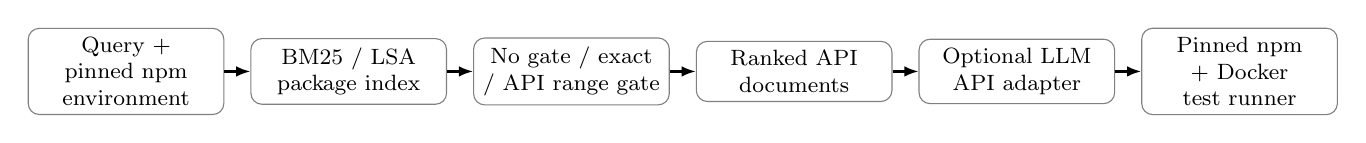
\begin{tikzpicture}[node distance=0.39cm and 0.33cm,
block/.style={draw=black!50,rounded corners,minimum height=.76cm,text width=2.25cm,font=\footnotesize,align=center},
arr/.style={-{Latex[length=1.8mm]},thick}]
\node[block] (task) {Query + pinned npm environment};
\node[block,right=of task] (index) {BM25 / LSA package index};
\node[block,right=of index] (gate) {No gate / exact / API range gate};
\node[block,right=of gate] (context) {Ranked API documents};
\node[block,right=of context] (llm) {Optional LLM API adapter};
\node[block,right=of llm] (exec) {Pinned npm + Docker test runner};
\draw[arr](task)--(index);
\draw[arr](index)--(gate);
\draw[arr](gate)--(context);
\draw[arr](context)--(llm);
\draw[arr](llm)--(exec);
\end{tikzpicture}
\caption{Extended implementation. Left four stages were evaluated; the generation adapter was dry-run to produce prompts, and the Docker npm executor was syntax-checked but not run in this environment.}
\label{fig:workflow}
\end{figure*}

The Python implementation loads documents, resolves the target version, constructs BM25 or LSA rankings, and applies the chosen constraint. The extension includes a provider-neutral chat-completions adapter which can emit CommonJS code from retrieved evidence using an explicitly supplied model and API key. It refuses to report generated code without a real response. Four example generation prompts were produced in dry-run mode; \emph{no hosted model was called}.

A separate Node.js executor defines four version-specific program tests covering Express wildcard routes, Express DELETE registration, and two removed Mongoose model methods. It prepares pinned npm dependencies and executes generated files only inside a Docker container with no network, read-only mounted workspace, resource caps, and no credentials. This runner is implemented but its real-package run is pending: Docker and the npm registry were not available in the execution environment. A separate 12-case Node.js test uses deliberately simplified \emph{local API emulations} only to verify subprocess execution and expected pass/fail handling; these cases must not be interpreted as tests of installed npm packages.

\section{Experimental Results and Discussion}
\subsection{Environment and Reproducibility}
We used Python 3.13.5, NumPy 2.3.5, scikit-learn 1.8.0, and Node.js 22.16.0 on CPU. Six new Python tests and the earlier 10 tests passed; the 12 scripted Node.js emulation cases matched their specified outcomes. The six ranking configurations shared the same 42 tasks and 39 documents. All corpus content, code, configuration, labels, raw task-level outcomes, and statistical scripts are provided in the project archive. There was no GPU inference or model API call.

\subsection{Retrieval Evaluation}
With $N$ tasks, we report correct-document Top-1 accuracy $N^{-1}\sum_i\mathbf{1}[r_{i1}=g_i]$, where $g_i$ is the hand-designated gold document; compatibility at rank one, $N^{-1}\sum_i C_{\mathrm{range}}(r_{i1},v_i)$; and Recall@3 / mean reciprocal rank computed against $g_i$. These distinguish target-version validity from finding the exact requested API. Table \ref{tab:results} reports observed scores.

\begin{table}[t]
\centering
\caption{Measured retrieval scores on 42 paired pilot tasks}
\label{tab:results}
\setlength{\tabcolsep}{3pt}
\begin{tabular}{lrrrr}
\toprule
Method & Top-1 & Valid@1 & R@3 & MRR@3\\
\midrule
BM25 & 42.9\% & 61.9\% & 81.0\% & .611\\
BM25 + exact & 66.7\% & 100\% & 90.5\% & .774\\
BM25 + range & 66.7\% & 100\% & 92.9\% & .790\\
LSA & 35.7\% & 52.4\% & 73.8\% & .536\\
LSA + exact & 57.1\% & 100\% & 90.5\% & .722\\
LSA + range & 57.1\% & 100\% & 88.1\% & .710\\
\bottomrule
\end{tabular}
\end{table}

\begin{figure}[t]
\centering
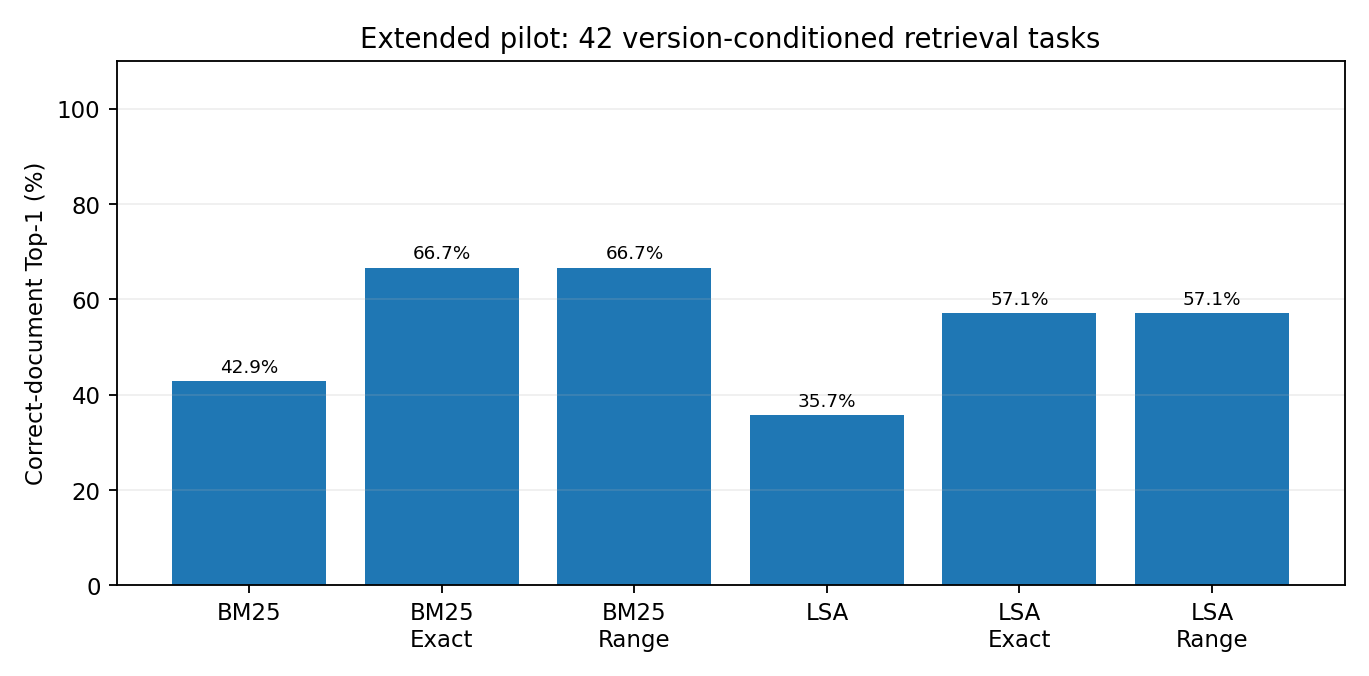
\includegraphics[width=\columnwidth]{../milestone3/retrieval_six_methods.png}
\caption{Observed correct-document Top-1 retrieval. The data are author-constructed and do not measure LLM generation.}
\end{figure}

Filtering increases the BM25 Top-1 count from 18/42 to 28/42 and the LSA count from 15/42 to 24/42. More importantly for the technical comparison, \emph{range-aware and exact-version filters tie on overall Top-1 accuracy}. On the six stable cross-version tasks, BM25 exact achieves 2/6 and BM25 range achieves 4/6; on the 36 migration tasks the corresponding counts are 26/36 and 24/36. Similarly, LSA improves on stable tasks from 1/6 to 3/6 but loses two hits on the migration subset. Therefore the range rule is capable of retaining cross-release evidence but is \emph{not} demonstrated to outperform simpler exact filtering overall.


\begin{table}[t]
\centering
\caption{Correct Top-1 hits by API type (stable 6, breaking 36)}
\label{tab:subgroups}
\setlength{\tabcolsep}{4pt}
\begin{tabular}{lrr}
\toprule
Method & Stable hits & Breaking hits\\
\midrule
BM25 + exact & 2/6 & 26/36\\
BM25 + range & 4/6 & 24/36\\
LSA + exact & 1/6 & 23/36\\
LSA + range & 3/6 & 21/36\\
\bottomrule
\end{tabular}
\end{table}

\subsection{Paired Statistical Analysis}
A task-level paired comparison between BM25 and BM25 + exact has 12 improvements and two regressions; the two-sided exact McNemar test gives $p=0.0129$. Resampling 21 API families (keeping both target versions together) with 10,000 fixed-seed replicates gives a 95\% cluster-bootstrap interval of roughly $[9.5,38.1]$ percentage points for the $23.8$-point difference. For BM25 exact versus range, there are two wins and two losses, giving $p=1.0$ and a zero-point mean difference. The analogous LSA gains are 21.4 points from the exact gate and zero from exact to range. These inferential calculations describe this small fixed fixture dataset; they are not evidence of an effect across real-world npm projects or independently sampled API changes.

\subsection{Baseline Reproduction and Execution Status}
The selected reference is DocPrompting \cite{docprompting}. The previous milestone reimplemented a simplified BM25 component on npm tasks. \emph{The published DocPrompting evaluation has not been reproduced}: its original Elasticsearch index, official tldr or CoNaLa splits, checkpoints, and matching generation metrics have not been run. Its publication-level numbers must not be compared with our different retrieval Top-1 percentages. The repository includes a faithful-reproduction procedure for a machine with suitable data, tools, and model weights.

The executable pipeline is more developed than at the previous milestone but has not yielded real npm-generated-code results. The four LLM prompts were generated without sending requests. The Docker runner was syntax checked, and twelve local emulation scenarios passed subprocess self-tests. We have \emph{not} installed Express, Mongoose, or React Router into the test harness in this environment; therefore no empirical Pass@1, real API failure-rate reduction, or completed RQ3 result is claimed. This is an explicit limitation relative to the course requirement to reproduce a base paper and develop an end-to-end model evaluation.


\subsection{Implementation Coverage and Remaining Dependencies}
Table \ref{tab:coverage} distinguishes implemented and measured stages from interfaces that are prepared but not validated with external tools. In particular, a syntactically valid execution runner is not evidence of a successful real-package experiment. This distinction is important for the course requirement to demonstrate substantial partial implementation without presenting planned experiments as completed findings.

\begin{table}[t]
\centering
\caption{Implementation status at this milestone}
\label{tab:coverage}
\setlength{\tabcolsep}{3pt}
\begin{tabular}{p{0.57\columnwidth}p{0.32\columnwidth}}
\toprule
Component & Status\\
\midrule
Dataset, lockfile parser, BM25 and LSA & Implemented and tested\\
Version-interval gate and six-method study & Implemented and measured\\
Statistical tests and plots & Implemented and measured\\
LLM API prompt and response adapter & Implemented; prompts dry-run\\
Isolated Docker/npm runner & Implemented; not executed\\
Full DocPrompting published reproduction & Not completed\\
Actual npm-generated-code Pass@1 & Not measured\\
\bottomrule
\end{tabular}
\end{table}

The remaining dependencies are explicit: access to official benchmark assets and a compatible legacy environment for DocPrompting, a permitted code-generation API or local model, npm registry access, and Docker for isolated execution. The source repository contains executable commands and input schemas for continuing these steps.

\subsection{Ablation and Validity Limitations}
The six conditions form a retrieval-stage ablation over the presence and type of compatibility constraint. The new stable-API tasks test the specific argument for ranges: cross-release documentation may still apply. However, the manually specified intervals encode prior knowledge and partly determine the compatibility metric, so 100\% Valid@1 after filtering is expected, not independently discovered compatibility. The dataset is small and author-labeled. The exact and range retrievers are compared with the same fixed corpus but no independent held-out test set. LSA is not a neural retriever, and the experimental corpus has only short paraphrases rather than complete official archived documentation. Execution emulations are not real library tests, and no LLM sampled code. Results do not establish superiority over industrial version-aware RAG services.


\subsection{Execution Protocol for the Next Evaluation Stage}
An executable research question requires a different unit of analysis from the retrieval pilot. A programming task will contain a target package and resolved version, a natural-language intent, a CommonJS module interface, and deterministic assertions. For each task, the research system will generate one solution under each retrieval condition. In addition to the six retrieval-stage configurations here, the full comparison will require a no-retrieval generator and an oracle condition supplied with independently verified target-version evidence. Every generator invocation must use the same named model, system instructions, decoding settings, input task, and output schema. The retrieved content itself is the treatment variable.

The real-package test runner will first install a specific npm release into its own workspace and preserve the resolved lockfile. It will not use an unpinned semver range. The generated module will then be evaluated in an isolated, network-disabled Docker container with a read-only mounted filesystem, bounded memory, CPU and process limits, and no secrets. For each solution, the harness should record package version, model identifier, retrieval condition, selected-document IDs, code, test assertions, exit status, timeout status, and a categorized failure cause. 
For the subsequent stage, the intended \emph{Pass@1} metric is:
\begin{equation}
 \mathrm{Pass@1}=\frac{1}{N}\sum_{i=1}^{N}\mathbf{1}[T(y_i)=\mathrm{pass}],
\end{equation}
Here $y_i$ is the first generated solution and $T$ is the task test suite. This formula defines the subsequent experiment; Pass@1 has not been measured. The current Docker runner has four task specifications; broader library coverage and a manual examination of test adequacy will be needed before generalization.

\subsection{Planned Conflict-Exposure Study}
RQ1 requires manipulating the amount of \emph{relevant but incompatible} API guidance while keeping retrieved context length and the desired task constant. We plan to use a fixed number $k$ of documentation chunks and choose independently verified compatible and incompatible items for the same API. The exposure fraction will be
\begin{equation}
 \gamma = \frac{\#\text{incompatible chunks in context}}{k}.
\end{equation}
With $k=4$, the values $\gamma\in\{0,0.25,0.5,0.75,1\}$ yield a controlled design. Matching the API identity is important: random unrelated text would test generic retrieval noise instead of version-conflicting evidence. To avoid changes in retrieval-score distribution acting as a hidden confounder, version-specific chunks should be comparable in length, prominence, and semantic relevance. Repeated paraphrases of one document are not independent observations and should not be treated as distinct real documentation sources. The future experiment must use real, separately sourced API guidance and version-pinned executable tests. \emph{No outcome for these conflict proportions is reported in this milestone.}

\subsection{Annotation and Reproduction Safeguards}
A critical distinction is that \emph{different publication versions are not automatically incompatible}. The same API call can remain valid across several releases, which motivated the three stable-API cases. In the larger dataset, compatibility should be assessed at the call-signature and behavioral level. Proposed verification involves checking vendor migration guides, archived API references, and executable counterexamples under both the old and target release. At least two independent annotators should review uncertain cases, with discrepancies resolved by a documented adjudication process. The final benchmark should separate APIs used in methodology development from a held-out set of packages or migrations, rather than reporting the accuracy of a system on the same items used to design its rules.

Faithful reproduction of DocPrompting is a separate dependency, not a by-product of these npm experiments. The authors' original sparse retrieval procedure requires a two-stage Elasticsearch index and their tldr data, whereas the present Python BM25 is a small adapted implementation. An adequate reproduction record will include the upstream commit, data and checkpoint hashes, exact environment versions, original evaluation scripts, the paper's corresponding reported metric, our measured value, and a reasoned deviation analysis. If the original model or index cannot be run, the result must remain labeled as an adaptation. This protects against comparing retrieval Top-1 on 42 npm tasks with generation Pass@k on unrelated published benchmarks.

\section{Conclusion and Future Work}
This extended milestone implements and tests six retrieval conditions, a semver-range API applicability constraint, an expanded 42-task corpus, paired significance analysis, a model prompt interface, and an isolated real-npm execution runner. The measured pilot supports the practical role of version constraints within a controlled retrieval corpus but does not show a net overall gain from API ranges over exact filtering. The remaining work is consequential: reproduce the original reference benchmark, validate API applicability on installed packages, replace paraphrases with archived authentic documentation, generate code with a pinned model, execute it in containers, vary incompatible evidence systematically (RQ1), and compute true Pass@1 and version-error rates (RQ3). A larger independently labeled study would also enable model and library generalization and cost and latency analysis. These steps must be completed before a final research paper can claim system-level effectiveness.

\balance
\begin{thebibliography}{99}
\bibitem{docprompting}
S. Zhou, U. Alon, F. F. Xu, Z. Wang, Z. Jiang, and G. Neubig, ``DocPrompting: Generating Code by Retrieving the Docs,'' in \emph{Proc. Int. Conf. Learn. Representations (ICLR)}, 2023. [Online]. Available: \url{https://openreview.net/forum?id=ZTCxT2t2Ru}.

\bibitem{coderag}
Z. Z. Wang, A. Asai, X. V. Yu, F. F. Xu, Y. Xie, G. Neubig, and D. Fried, ``CodeRAG-Bench: Can Retrieval Augment Code Generation?,'' in \emph{Findings Assoc. Comput. Linguistics: NAACL}, 2025, pp. 3199--3214, doi: 10.18653/v1/2025.findings-naacl.176.

\bibitem{libevolution}
S. Kuhar, W. U. Ahmad, Z. Wang, N. Jain, H. Qian, B. Ray, M. K. Ramanathan, X. Ma, and A. Deoras, ``LibEvolutionEval: A Benchmark and Study for Version-Specific Code Generation,'' in \emph{Proc. NAACL}, 2025, pp. 6826--6840, doi: 10.18653/v1/2025.naacl-long.348.

\bibitem{gitchameleon}
D. Misra, N. Islah, V. May, B. Rauby, Z. Wang, J. Gehring, A. Orvieto, M. S. Chaudhary, E. B. Muller, I. Rish, S. E. Kahou, and M. Caccia, ``GitChameleon 2.0: Evaluating AI Code Generation Against Python Library Version Incompatibilities,'' in \emph{Proc. ACL}, 2026, pp. 46792--46831, doi: 10.18653/v1/2026.acl-long.2170.

\bibitem{npmchanges}
D. Kong, J. Liu, L. Bao, and D. Lo, ``Toward Better Comprehension of Breaking Changes in the NPM Ecosystem,'' \emph{ACM Trans. Softw. Eng. Methodol.}, vol. 34, no. 4, Art. no. 111, pp. 1--23, 2025, doi: 10.1145/3702991.

\bibitem{gullible}
G. Hong, J. Kim, J. Kang, S.-H. Myaeng, and J. J. Whang, ``Why So Gullible? Enhancing the Robustness of Retrieval-Augmented Models against Counterfactual Noise,'' in \emph{Findings Assoc. Comput. Linguistics: NAACL}, 2024, pp. 2474--2495, doi: 10.18653/v1/2024.findings-naacl.159.

\bibitem{express}
Express.js, ``Upgrading to Express 5,'' [Online]. Available: \url{https://expressjs.com/en/guide/migrating-5/}. Accessed: Nov. 8, 2026.

\bibitem{mongoose}
Mongoose, ``Migrating from 6.x to 7.x,'' [Online]. Available: \url{https://mongoosejs.com/docs/7.x/docs/migrating_to_7.html}. Accessed: Nov. 8, 2026.

\bibitem{router}
React Router, ``Upgrading from v5,'' [Online]. Available: \url{https://reactrouter.com/docs/en/v6/upgrading/v5}. Accessed: Nov. 8, 2026.

\end{thebibliography}
\end{document}
